\section{\Acrfullpl{ffn}}

Les réseaux de neurones profonds sont parmi les modèles les plus expressifs en \acrshort{ml}.
Leur succès pratique est incomparable aux modèles qui les ont précédés, 
que se soit en termes de qualité des résultats ou de variétés de domaines d'application.
De plus, grâce aux théorèmes dits d'approximation universelle, ce succès empirique est formellement assuré.

Les \acrshort{ffn} sont l'architecture neuronale la plus simple et la plus utilisée.
Mathématiquement, un réseau de neurones feed-forward de profondeur \(\ell\) 
peut être vu comme une fonction \(f\) telle que :

\begin{equation}
    \label{eq:ffn}
    f = h_1 \circ \varphi_1 \circ h_2 \circ \varphi_2 \circ \cdots \circ h_\ell \circ \varphi_\ell
\end{equation}
où les \(h_i\) sont des applications affines et les \(\varphi_i\) sont des applications non linéaires.

Le réseau de neurones défini par l'équation~\ref{eq:ffn} 
est souvent représenté par un graphe orienté acyclique (voire Figure~\ref{fig:ffn}).

\begin{figure}[hbt]
    \begin{center}
        \def\layersep{2.5cm}

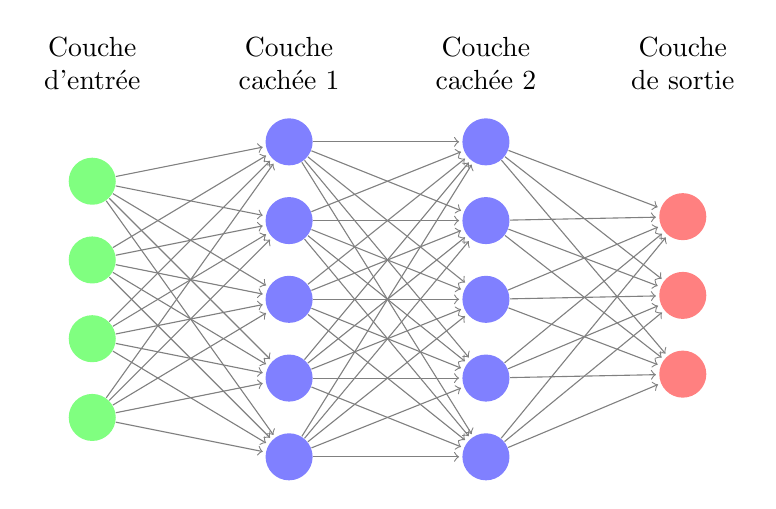
\begin{tikzpicture}[shorten >=1pt,->,draw=black!50, node distance=\layersep]
    \tikzstyle{every pin edge}=[<-,shorten <=1pt]
    \tikzstyle{neuron}=[circle,fill=black!25,minimum size=17pt,inner sep=0pt]
    \tikzstyle{input neuron}=[neuron, fill=green!50];
    \tikzstyle{output neuron}=[neuron, fill=red!50];
    \tikzstyle{hidden neuron}=[neuron, fill=blue!50];
    \tikzstyle{annot} = [text width=4em, text centered]

    % Draw the input layer nodes
    \foreach \name / \y in {1,...,4}
    % This is the same as writing \foreach \name / \y in {1/1,2/2,3/3,4/4}
        \node[input neuron] (I-\name) at (0,-\y) {};

    % Draw the hidden layer nodes
    \foreach \name / \y in {1,...,5}
        \path[yshift=0.5cm]
            node[hidden neuron] (H1-\name) at (\layersep,-\y) {};

    \foreach \name / \y in {1,...,5}
        \path[yshift=0.5cm]
            node[hidden neuron] (H2-\name) at (\layersep*2,-\y) {};

    % Draw the output layer node
    \foreach \name / \y in {1,...,3}
    % This is the same as writing \foreach \name / \y in {1/1,2/2,3/3,4/4}
        \path[yshift=-0.45cm]
            node[output neuron] (O-\name) at (\layersep*3,-\y) {};
    

    % Connect every node in the input layer with every node in the
    % hidden layer.
    \foreach \source in {1,...,4}
        \foreach \dest in {1,...,5}
            \path (I-\source) edge (H1-\dest);

    \foreach \source in {1,...,5}
        \foreach \dest in {1,...,5}
            \path (H1-\source) edge (H2-\dest);
    % Connect every node in the hidden layer with the output layer
    \foreach \source in {1,...,5}
        \foreach \dest in {1,...,3}
            \path (H2-\source) edge (O-\dest);

    % Annotate the layers
    \node[annot,above of=H1-1, node distance=1cm] (hl) {Couche cachée 1};
    \node[annot,above of=H2-1, node distance=1cm] (h2) {Couche cachée 2};

    \node[annot,left of=hl] {Couche d'entrée};
    \node[annot,right of=h2] {Couche de sortie};
\end{tikzpicture}
    \end{center}
    \caption{Un réseau de neurone \acrshort{ffn} de profondeur 3.}
    \label{fig:ffn}
\end{figure}
